\documentclass[preprint,12pt,a4paper]{elsarticle}
\pdfinfoomitdate=1\pdftrailerid{}
\usepackage{amssymb,amsmath,booktabs,array,float,hyperref,xurl,placeins}
\newcolumntype{P}[1]{>{\raggedright\arraybackslash}p{#1}}
\setlength{\parindent}{0pt}\setlength{\emergencystretch}{1.5em}
\clubpenalty=10000\widowpenalty=10000
\setlength{\abovecaptionskip}{9pt}\setlength{\belowcaptionskip}{8pt}
\hypersetup{hidelinks}\journal{SoftwareX}
\renewcommand{\topfraction}{.9}\renewcommand{\textfraction}{.05}\renewcommand{\floatpagefraction}{.8}
\renewcommand{\bibfont}{\footnotesize}
\setlength{\bibsep}{0pt}
\begin{document}\begin{frontmatter}
\title{WorkCert: Reconstruction error metadata for force--displacement tables}
\author[a]{Saisai Hou}\author[a]{Yunzhi Zhu}\author[a]{Sen Zhang\corref{cor}}
\cortext[cor]{Corresponding author.}\ead{szhang@niit.edu.cn}
\affiliation[a]{organization={Department of Public Basic Courses, Nanjing University of Industry Technology},city={Nanjing},country={China}}
\begin{abstract}
WorkCert is a Python package for reduced force--displacement tables with reconstruction-error metadata and reusable work queries. Compensated integration and local range sums support long references and short windows. Examples using public data demonstrate energy-absorption screening, selective refinement, work-to-stroke inversion and signed cyclic histories. Refinement identifies the leading candidate at reported masses; mass rounding leaves the comparison unresolved. Six selectors and objective-matched dynamic programming contextualize reduction quality. Within work-priority selection, direct interval-error stopping reduces median table size from 27 to 14 nodes for the same 1\% requirement. Source data, tests, numerical outputs and article-building inputs accompany the software.
\end{abstract}
\begin{keyword}Research software\sep Force--displacement data\sep Reconstruction error\sep Energy absorption\sep Stable integration\sep Cyclic response\end{keyword}
\end{frontmatter}\clearpage
\section*{Required Metadata}\section*{Current code version}
\begin{table}[H]\small\centering
\begin{tabular}{|P{.05\linewidth}|P{.39\linewidth}|P{.425\linewidth}|}\hline
\textbf{Nr.}&\textbf{Code metadata description}&\textbf{Metadata}\\\hline
C1&Current code version&0.3.0\\\hline
C2&Permanent GitHub link to code/repository used for this code version&\url{https://github.com/changs1723/WorkCert/tree/v0.3.0}\\\hline
C3&Legal Code License&MIT License\\\hline
C4&Code versioning system used&Git\\\hline
C5&Software code languages, tools, and services used&Python; NumPy; command-line interface\\\hline
C6&Compilation requirements, operating environments \& dependencies&Python $\geq$3.10; NumPy $\geq$1.24. No compiled runtime extension. Research dependencies are separate.\\\hline
C7&If available Link to developer documentation/manual&\url{https://github.com/changs1723/WorkCert/blob/v0.3.0/software/docs/API.md}\\\hline
C8&Support email for questions&\href{mailto:szhang@niit.edu.cn}{szhang@niit.edu.cn}\\\hline
\end{tabular}\caption{Code metadata.}\end{table}

\section{Motivation and significance}
Structural response tables support subsequent calculations. The Abaqus bushing example transfers detailed force--motion histories into connector definitions for assembly analysis \cite{AbaqusBushing}. Experimental databases similarly support stroke-dependent energy absorption (EA), specific energy absorption (SEA), mean crushing force (MCF) and crush-force efficiency (CFE). A reusable representation should retain its numerical error information when its source is unavailable to the consumer.

Ramer, Douglas--\allowbreak Peucker, Visvalingam--\allowbreak Whyatt and time-series segmentation provide established simplification strategies \cite{Ramer1972,DouglasPeucker1973,Visvalingam1993,Keogh2001}. Optimal approximation depends on the objective \cite{Imai1988}; area measures have their own established theory \cite{Bose2006,Daneshpajouh2012}. WorkCert integrates continuous work-error extrema, stable queries, serialization, source identity and directed branches. External nodes from \path{rdp}, \path{simplification} or \path{shapely.simplify} share this interface \cite{rdpSoftware,Hugel2021,ShapelySoftware}. The resulting tables retain common query and verification operations across selectors.

\section{Software description}
\subsection{Software architecture}
NumPy is the sole runtime dependency. Modules separate validation, selection, error evaluation, queries, persistence and chronological branches. Immutable arrays protect cached sums. JSON stores retained nodes, native-unit labels, reconstruction errors and source fingerprints in a versioned schema. The producer accesses the dense reference; the consumer loads only the exchanged table and its metadata.

\subsection{Software functionalities}
Let $F$ be the supplied piecewise-linear (PL) reference on $[0,U]$ and $\widehat F$ its $K$-node interpolant. Define $r=F-\widehat F$ and $D(u)=\int_0^u r(s)\,ds$. The ideal PL reconstruction quantities are
\begin{align}
\eta&=\int_0^U|r(s)|\,ds,&\xi&=(\eta+|D(U)|)/2,\\
E_p&=\max|D|,&E_w&=\max D-\min D,\qquad\delta=\max|r|.
\end{align}
An interval's work error is $D(b)-D(a)$, hence $E_p\leq E_w\leq\xi\leq\eta$. For positive and negative residual areas $P,N$, $\xi=\max(P,N)$. Reference nodes and interior zeros of $r$ locate continuous extrema.

Three numerical layers have distinct meanings. The quantities above measure representation error. Float64 quadrature, interpolation and output rounding introduce arithmetic error, which these bounds do not enclose. Source verification checks identity and numerical consistency: hashes and retained coordinates match exactly; nonzero numerical fields allow 16 units in the last place (ULPs), while zero must match zero. This field-local comparison is a consistency policy, not an outward-rounded enclosure. Measurement uncertainty belongs to the underlying experiment.

Residuals are evaluated in local force offsets. A compensated balanced scan accumulates trapezoid terms in $O(n)$ work and storage, with \path{math.fsum} for the terminal sum. Queries integrate endpoint pieces and cached interior ranges rather than subtracting global prefixes. Cached range queries cost $O(\log K)$; a cancellation diagnostic invokes direct summation when needed, costing $O(K)$. Derived overflow raises \path{ValueError}; the command-line interface returns status 2 with a concise diagnostic.

Users choose work priority, vertical priority, effective-area Visvalingam--Whyatt or uniform sampling. The priority methods share the largest-residual split but rank intervals differently. Endpoints and a chosen absolute, positive or negative peak are retained. Labels specify units without rescaling; mm and kN give J. Relative bounds use $|W(U)|$; zero terminal work requires absolute tolerances.

Adaptive construction maintains interval summaries $(d,l,h)$: terminal residual work and its minimum and maximum, together with area and force deviation. Concatenation gives
\begin{equation}
d=d_A+d_B,\quad l=\min(l_A,d_A+l_B),\quad h=\max(h_A,d_A+h_B).
\end{equation}
Only new intervals and their balanced-tree ancestors change after insertion. Updates cost $O(\log K)$, tree storage is $O(K)$, and residual rescanning retains $O(nK)$ worst-case work. A final full evaluation checks the selected table. Greedy refinement can increase an error, so stopping evaluates every representation. VW selection costs $O(n\log n)$.

\begin{minipage}{\linewidth}
\subsection{Sample code snippets}
The producer creates an absolute 1 J interval-work table; the consumer needs no dense reference:
\begin{verbatim}
from workcert import reduce_response, ReducedResponse
import numpy as np
a = np.loadtxt("data/prepared/PLA_STWC-1.csv",
               delimiter=",", skiprows=1)
t = reduce_response(a[:, 0], a[:, 1], method="work",
    max_points=129, tolerance=1., certificate="window",
    x_unit="mm", force_unit="kN")
t.save("response.json")
c = ReducedResponse.load("response.json")
energy = c.window_work(10., 20.)
error = c.certificate.window
met_budget = c.metadata["tolerance_met"]
\end{verbatim}
\end{minipage}
The consumer can request finer source tables when error intervals overlap. \path{from_indices} accepts externally selected nodes; \path{split_monotone_branches} retains reversals, direction and zero-work dwell events.

\subsection{Verification and AI-assisted implementation}
The installed suite contains 81 methods, including analytical acceptance cases and constant, affine, cancellation, rescaling, persistence and overflow regressions. Both published distribution formats passed all 81 tests in six new Windows environments with Python 3.10/3.12/3.14 and NumPy 2.2.6/2.3.5/2.5.4. The Python 3.12 environments reused base dependencies. The version-tag workflow passed all 15 Linux/macOS/Windows and Python 3.10--3.14 jobs, each including the installed suite, 12 branch-summary tests and four verification-CLI tests. It also installed and tested the built wheel and source distribution. Exact-rational fixtures and an independent scalar integrator check reconstruction and queries; small dynamic-programming problems are checked against enumeration. Frozen-table identity checks are recorded separately from independent numerical recalculation.

OpenAI Codex (OpenAI; local CLI version 0.166.0-alpha.5.1) assisted research planning, public-data collection, implementation, analysis, plotting and manuscript preparation. The assisted code includes \path{software/src/workcert}, \path{validation} and \path{authoring}. The script \path{validation/reproduce_v03.py} verifies saved results; \path{authoring/build_documents_v03.py} rebuilds the article and data-derived figures. The dated contributor-verification record identifies human checks. Expected values use analytical or rational calculations and original workbook indicators.

\section{Illustrative examples}
\subsection{Integration and verification precision}
A 100,001-point constant reference, $x_i=10^{-4}i$ mm and $F_i=0.1$ kN, reduces to two endpoints with zero reconstruction error and 1 J terminal work. Constant and affine regressions vary sequence length and coordinate and force scales. For one million intervals, the computed source work differs from the correctly rounded exact binary-input integral by one ULP (Fig.~\ref{fig:numeric}).

For $x=[0,1,2]$ and $F=[10^{16},0,1]$, full-node retention gives $E_w=0$, yet subtracting rounded global prefixes loses the 0.5 J window $[1,2]$. Direct integration returns 0.5 J. A signed unit-step fixture $F=[0,10^{16},1,-10^{16},0]$ returns 1 J by retaining both components of each endpoint mean. A separate $10^{12}$-baseline example has $E_p=0.010009765625$ J; replacing its error metadata by zeros is rejected. These cases distinguish stable computation from representation fidelity.

\begin{figure}[!htbp]\centering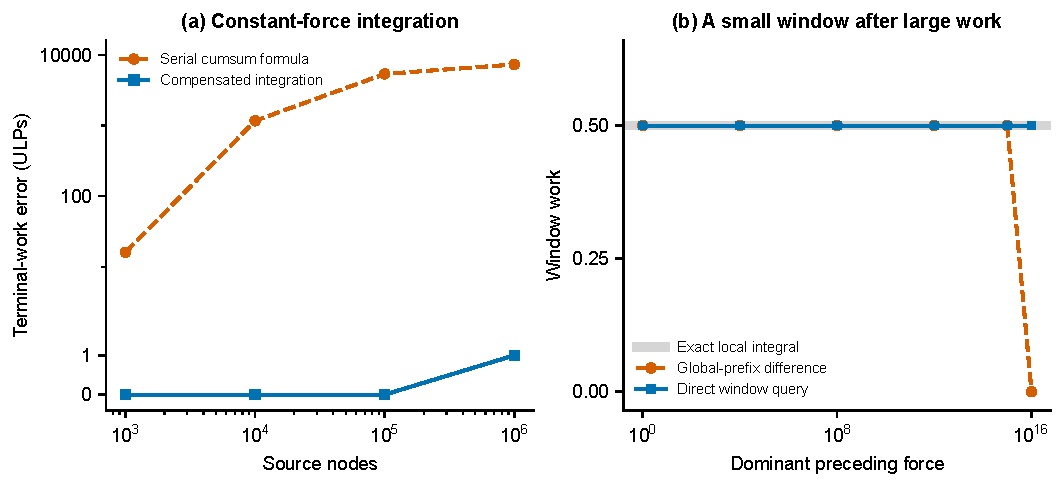
\includegraphics[width=\linewidth]{figures/fig01_numerics.pdf}
\caption{Arithmetic tests: (a) terminal-work error against exact binary-input integration; (b) local-window work with a dominant preceding force. Serial accumulation and prefix subtraction are explicit comparison formulas. OpenAI Codex assisted with the archived plotting code.}\label{fig:numeric}\end{figure}

\subsection{Decision-focused table exchange}
The PLA+ dataset contains 40 singly tested configurations and two triplicate controls: 42 configurations and 46 specimens \cite{Saber2026,Guler2026}. A demonstration 1 J interval budget retains 1520 of 46,000 source nodes. At stroke $u$, $EA=W(u)$, $SEA=EA/m$, $MCF=EA/u$ and $CFE=MCF/P(u)$ for prefix peak $P(u)$. Retaining the source global peak makes later peak queries exact, sharpening CFE intervals to $(\widehat W\pm E_p)/(uP)$; earlier queries use force-error bounds and retained anchors, with a positive peak lower bound.

All 184 indicator sets contain their dense-reference values. The same two three-specimen controls are queried at four strokes, giving eight descriptive scatter comparisons, not eight independent experiments. The closest prefix-bound/SD ratio is 0.921 at nominal SCMC, 10 mm. Control-mean intervals average specimen endpoints without a $\sqrt3$ reduction. A $\pm0.05$ g mass-rounding scenario changes SEA by at most 0.310\%.

The initial tables separate 3345 of 3444 configuration pairs, but only 103 of 164 adjacent pairs in dense-reference order. At 20 mm, configurations 26 and 35 overlap. A consumer first selects the largest lower bound, then requests that leader and every rival whose upper bound reaches it. This selects only 26 and 35, without dense-reference ranking. At the reported masses, halving their budgets to 0.5 J identifies configuration 26 as the leader: its lower bound exceeds every competing upper bound by 0.00953 kJ/kg. Total retained nodes become 1538, a net increase of 18; the two replacement tables transmit 81 nodes, while 44 tables remain unchanged. Subsequent source evaluation gives a best--runner-up gap of 0.02340 kJ/kg.

With $\pm0.05$ g mass rounding, configurations 26 and 35 overlap again. Even the full source curves give a worst-case SEA difference of $-0.00344798$ kJ/kg. Further curve refinement cannot resolve this comparison without more precise masses.

The same interface answers an inverse query. A 20-node STWC-1 table maps 100 J prescribed work into $[21.812,22.170]$ mm, containing the reference value 22.017 mm. Inversion is restricted to the positive-force 10--40 mm loading interval. It queries quasi-static work capacity, rather than predicting impact dynamics (Fig.~\ref{fig:workflow}).

Source-indicator checks cover 45/46 workbook EA, SEA, MCF and CFE entries, and all peaks. Specimen 05's stated 50 mm EA differs because its workbook integrates to 50.009 mm. Actual endpoints of 50.004--50.009 mm explain all 13 nonzero EA discrepancies; these checks concern source calculations and endpoint conventions.

\begin{figure}[!htbp]\centering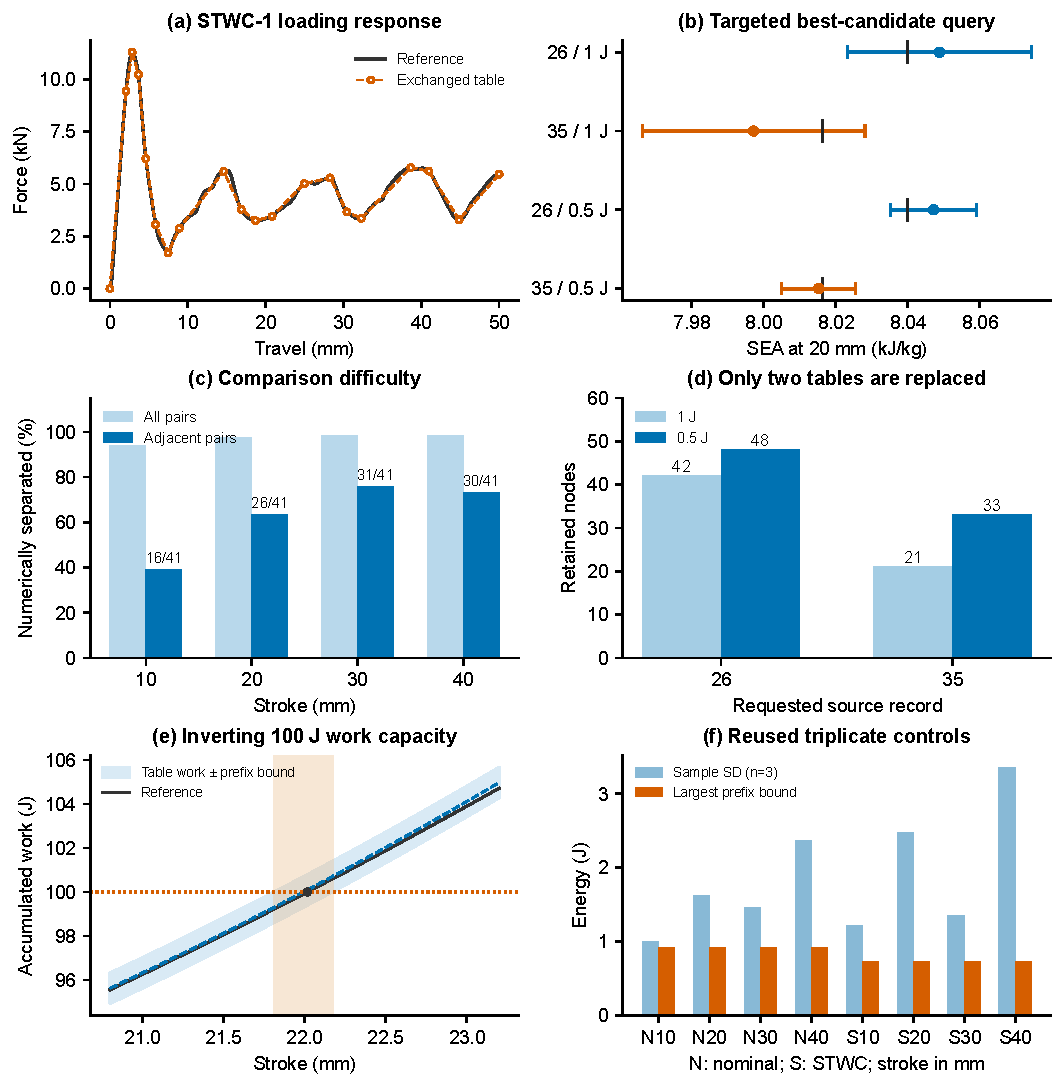
\includegraphics[width=\linewidth]{figures/fig02_decisions.pdf}
\caption{Consumer workflow: reference/table response, candidate intervals at reported masses, adjacent versus all-pair separation, targeted point allocation, inverse work query and repeated-specimen scatter. Black ticks in (b) mark reference values used only for evaluation. OpenAI Codex assisted with the archived plotting code.}\label{fig:workflow}\end{figure}

A connector exchange uses 33 vertical-priority nodes, with $\delta=0.204$ kN, $E_p=0.665$ J and $E_w=0.815$ J. A separate reader verifies exported force--displacement rows and work queries. This example evaluates loading-table exchange; solver response, unloading and convergence require their own constitutive analysis.

\subsection{Signed cyclic response}
A stainless-steel record contains 125,157 chronological pairs \cite{CyclicDataset2024,CyclicPaper2022}. Preprocessing retains 2971 monotone branches and 1984 dwell events; branch-size quartiles are 2, 9 and 26 nodes. A diagnostic deadband detects 94 reversals across 0.1--5 mm, consistent with the 47-cycle S1-L1 failure in Table~3 of \cite{CyclicPaper2022}. The original path remains unchanged.

Work-priority branches use absolute-peak retention, a 129-point cap and budget $0.001|W_b|$. They retain 13,890 nodes. Branch 2533 reaches the cap with $E_w=0.154$ J against 0.087 J requested, a 1.769 ratio; \path{tolerance_met=False} exposes this outcome. Against 92.034 kJ signed path work, terminal error is 68.530 J, continuous chronological error 68.72 J and summed branch-window bound 104.48 J. These are computed global results, not an automatic consequence of relative branch budgets. Descending summaries become $(-d,l-d,h-d)$ before chronological composition. The standalone composer evaluates this real-arithmetic identity with sequential float64 operations; its metadata exclude rounding error. Path work differs from closed-cycle dissipation.

\begin{figure}[!htbp]\centering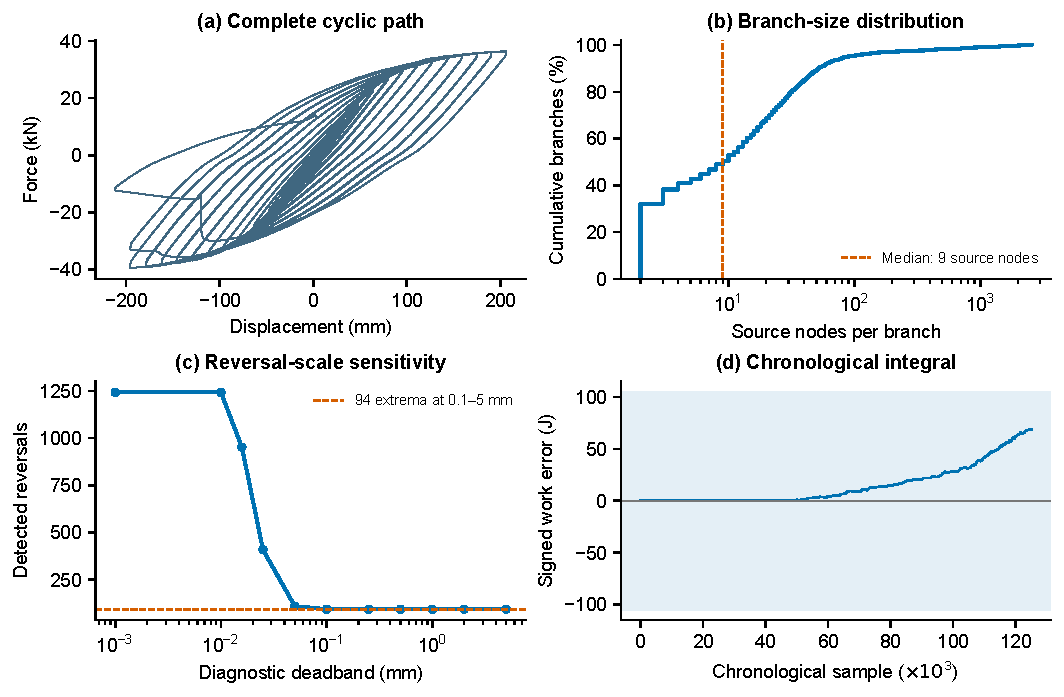
\includegraphics[width=\linewidth]{figures/fig03_cyclic.pdf}
\caption{Cyclic path, branch sizes, diagnostic reversal scales and chronological work error. Shading shows $\pm\sum_b E_{w,b}$. OpenAI Codex assisted with the archived plotting code.}\label{fig:cyclic}\end{figure}

\subsection{Selectors and matched-objective controls}
The comparison comprises 23 CX-steel honeycomb records, one enhanced double-arrow honeycomb (EDAH) record and 46 PLA+ curves \cite{Afkhami2022,Afkhami2023,AfkhamiDataset2022,WuDataset2025,Wu2026,Saber2026}. Archived preparation includes CX contact alignment at 0.5 kN and a window ending at 40\% of nominal loaded size. Six selectors use 9, 17, 33, 65 and 129 nodes. Fixed-count RDP uses normalized coordinates; native tolerance selectors are cross-checked separately. Outputs comprise 2100 force tables, 350 work-only tables, 560 stopping cases and 70 scalar controls.

The pooled 33-node median favors VW, whereas CX alone favors vertical priority and EDAH favors work priority. Equal-cohort and equal-configuration weighting retain VW as the lowest aggregate window median; the single EDAH record still limits that cohort's evidence. Explicit method choice therefore remains part of the API (Fig.~\ref{fig:selectors}).

\begin{table}[!htbp]\small\centering
\caption{Median 33-node work errors normalized by $|W(U)|$ over 70 references: 23 CX, 1 EDAH and 46 PLA+. Optimality ratios use 58 references ($n\leq1000$): 12 CX and 46 PLA+, without EDAH. Uniform sampling lacks the common peak constraint and is excluded from ratios.}\label{tab:selectors}
\begin{tabular}{lrrrr}\toprule Selector&$E_p$ (\%)&$E_w$ (\%)&$\eta/\eta^*$&$\delta/\delta^*$\\\midrule
Work priority & 0.168 & 0.207 & 1.319 & 2.615 \\
Vertical priority & 0.204 & 0.239 & 1.370 & 1.663 \\
RDP, fixed count & 0.243 & 0.281 & 1.577 & 5.632 \\
Visvalingam--Whyatt & 0.155 & 0.187 & 1.396 & 3.096 \\
Uniform + peak & 0.229 & 0.344 & 2.657 & 10.351 \\
Uniform & 0.231 & 0.364 & -- & -- \\
\bottomrule\end{tabular}\end{table}

Dynamic programming supplies 580 area- or force-optimal paths under identical endpoint and peak constraints across all five budgets. Work priority's area-cost ratio and vertical priority's force-cost ratio address different objectives; neither establishes prefix-error optimality.

\begin{figure}[!htbp]\centering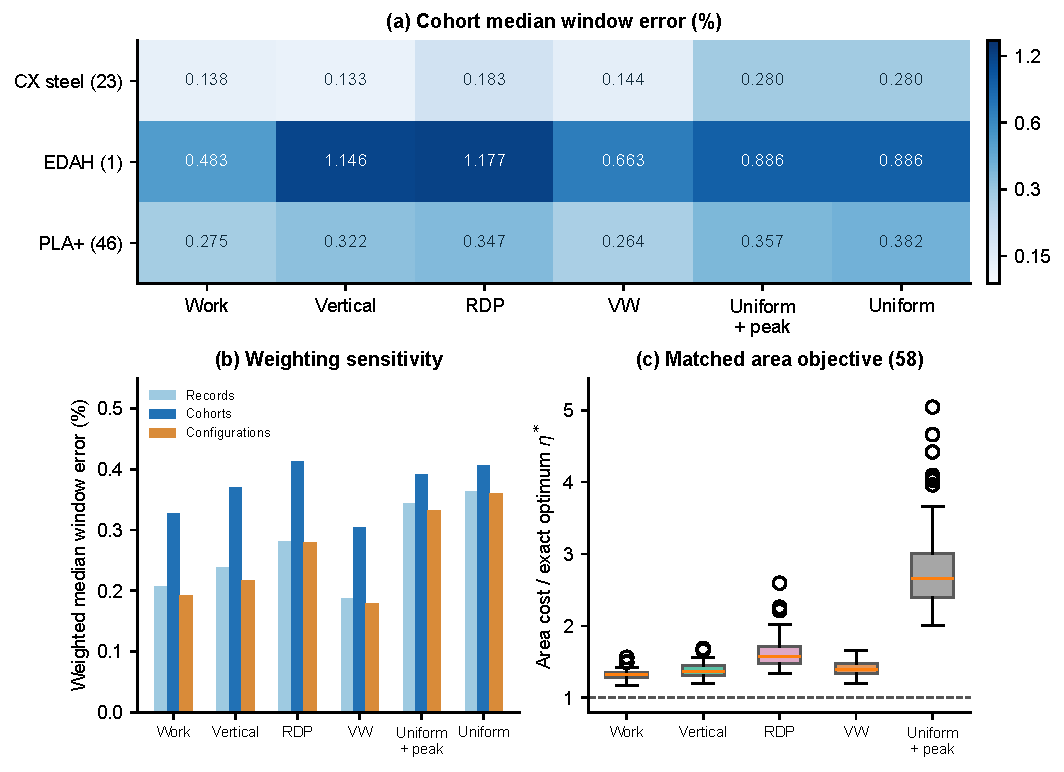
\includegraphics[width=\linewidth]{figures/fig04_selectors.pdf}
\caption{Cohort-specific window errors, weighting sensitivity and matched-area optimality gaps. OpenAI Codex assisted with the archived plotting code.}\label{fig:selectors}\end{figure}

\subsection{Stopping and scale}
For the same 1\% interval-work requirement, work-priority stopping retains median 14 nodes using $E_w$, versus 27 using conservative $\eta$. This compares stopping measures within one selector. Prefix-only requirements are tabulated separately.

Synthetic scaling uses $10^3$--$10^6$ samples and three tolerances on Windows 10, an 11th Gen Intel Core i5-11300H @ 3.10GHz CPU, 15.69 GiB RAM, Python 3.12.14 and NumPy 2.3.5. At one million samples and 0.1\% window tolerance, three independent paired processes give median 11.78 s for full-scan version 0.1 and 4.88 s for the current stable incremental implementation, retaining 107 nodes. Complete error evaluations decrease from 105 to 1. Small cases incur tree and compensated-sum overhead. Figure~\ref{fig:scale} reports this signal and host, with source hashes and individual timings archived.

\begin{figure}[!htbp]\centering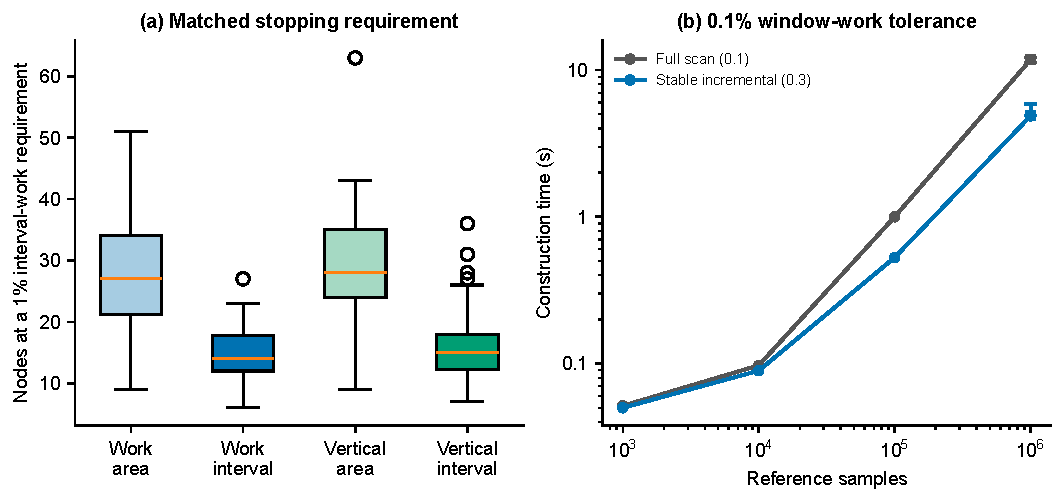
\includegraphics[width=\linewidth]{figures/fig05_scaling.pdf}
\caption{Matched interval stopping and measured construction cost. Boxes show quartiles and medians, with 1.5-interquartile-range whiskers; timing bars show three-process minimum--maximum ranges. OpenAI Codex assisted with the archived plotting code.}\label{fig:scale}\end{figure}

\FloatBarrier
\section{Impact}
Database curators can exchange a response once, support changing work limits, and refine only records that obstruct a requested comparison. The best-candidate example separates representation error from input precision: targeted refinement resolves the reported-mass comparison, while mass rounding identifies the need for better measurements. Inverse work queries reuse the same metadata.

Structural analysts can inspect both force fidelity and work error before using a loading table. Researchers comparing simplifiers can import their own nodes, while cyclic-data users compose branch summaries without reloading the full reference. Full source exchange remains practical for these small databases; the reduced-table interface supplies explicit error accounting and selective refinement. Independent laboratory adoption and solver-level effects remain open evaluation tasks.

\section{Conclusions}
WorkCert integrates reconstruction errors, compensated work queries, persistence and directed branches. Local range integration handles short-window cancellation; field-local checks test metadata without a source-force error floor. Decision-driven refinement connects point budgets to a specific candidate query. The frozen article snapshot binds this demonstration to its software, data and build inputs.

\section*{CRediT authorship contribution statement}
\textbf{Saisai Hou:} Conceptualization, Methodology, Software, Formal analysis, Visualization, Writing -- original draft.
\textbf{Yunzhi Zhu:} Methodology, Validation, Data curation, Writing -- review \& editing.
\textbf{Sen Zhang:} Conceptualization, Supervision, Resources, Writing -- review \& editing, Project administration.
\section*{Declaration of competing interest}
The authors declare no competing interests.
\section*{Funding}
This work was supported by the General Program of Natural Science Research (Basic Science) in Higher Education Institutions of Jiangsu Province (Grant No. 25KJD110002).
\section*{Acknowledgements}
The authors thank the contributors of the public compression and cyclic-loading datasets.
\section*{Data and code availability}
The CC BY 4.0 sources are \url{https://doi.org/10.17632/8bxkdw4nfw.1}, \url{https://doi.org/10.5281/zenodo.16399749}, \url{https://doi.org/10.17632/v7p6y654ft.4} and \url{https://doi.org/10.5281/zenodo.10829958}. The fixed software source is \url{https://github.com/changs1723/WorkCert/tree/v0.3.0}. The software archive is \url{https://doi.org/10.5281/zenodo.23934502}.  The final article sources, figures and build inputs are fixed at \url{https://github.com/changs1723/WorkCert/tree/article-v0.3.0-final}.  The article manifest links the final PDF and editable sources to their software modules and scientific inputs. Verification and recomputation are separate documented commands.
\section*{Declaration of generative AI and AI-assisted technologies in the manuscript preparation process}
OpenAI Codex (OpenAI; local CLI version 0.166.0-alpha.5.1) assisted with research planning, literature and public-data collection, implementation and debugging, numerical analysis and verification, figure preparation, drafting, language editing and typesetting. The authors are responsible for the research design, interpretation, software, results and final manuscript.
\bibliographystyle{elsarticle-num}{\small\bibliography{references}}
\end{document}
